\documentclass[a4paper]{article}

\input defi2
\renewcommand{\red}[1]{#1}
\usepackage{chemarrow}
\urlstyle{same}

\newcommand{\tocheck}{\marginpar{\small to check}}


\title{P3M User Manual}
\author{}
\date{}
\begin{document}
\maketitle

\section{Calling the system}
\label{sec:call}

\red{The system  P3M takes as input files representing MIMs as created by 
PathVisio\footnote{\url{https://github.com/PathVisio/pathvisio}}. Arrow
types allowed in the file are: 
{\em necessary stimulation} %  ($\Aactiv$ or $\Nactiv$),
 (~$\Nactiv$),  {\em
  conversion} ($\Aprod$), {\em inhibition}
($\Ainhib$) and {\em binding} ($\chemarrow$). This latter type of
arrow is used when the left hand side of a
production/activation/inhibition is a set of
entities. In other terms,  nodes labelled by sets of
entities, like in Figure \ref{fig:actinh}(a), are replaced by a set of
nodes linked by the binding arrow, like shown in
 Figure \ref{fig:actinh}(b). This makes it easier for the user to
 select entity types and initial values by use of the graphical
 interface (described below).
}

\begin{figure}[htb]
\begin{center}
\begin{tabular}{ccc}
    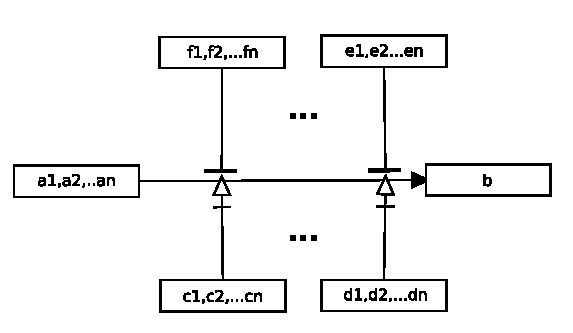
\includegraphics[scale=0.5]{actinh-notitle.pdf} &~~&
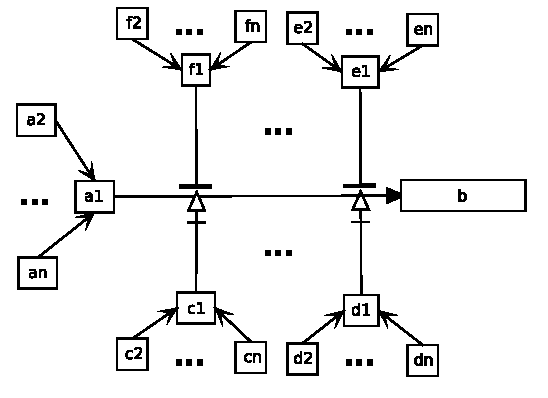
\includegraphics[scale=0.5]{actinh2.pdf} \\
(a) && (b)
\end{tabular}
\end{center}
\caption{Activations/Inhibitions}
\label{fig:actinh}
\end{figure}

The system P3M is called from the command line with the following syntax:
\begin{verbatim}
    p3m [<options>] 
\end{verbatim}
The possible options (shown when the system is called with the {\tt
  -help} option) are:
\begin{description}
\item[-filename] This option is followed by the name of 
 the Pathvisio file (without the {\tt
  .gpml} extension). If not set, the system tries to open the file 
file {\tt example.gpml}.
 \item[-grounding] This option is followed by a natural number,
   representing the time up to which the LTL encoding of the theory is
   grounded. Its default value is $0$.
\item[-query] This option is followed by the query passed to the
  system for either graph querying or graph updating. The query is a
  string starting with either the character {\tt +} or the character 
$\thicksim$. %  {\tt \textasciitilde}.
 The {\tt +} character identifies positive
  queries, and   $\thicksim$ %{\tt \textasciitilde} 
represents negation.
The positive/negative character is 
 followed by the name of an entity
  occurring in the graph and the time at which the literal (positive
  or negative atom) is required to hold. The integer representing time
  is enclosed  in
  round brackets. All special symbols (including
  brackets) must be escaped (i.e. preceded by a backslash).

For instance, P3M can be called with the options:
\begin{verbatim}
        -query +Galactosidase\(5\) 
        -query ~Galactosidase\(5\) 
\end{verbatim}

If the {\tt -query} option is missing, P3M only checks the validity of the graph.


\item[-assumed] This option is used when the user wishes to set
  initial values for some variables. The option is followed by a
  string containing a sequence of ``literals'', i.e. entity names
  preceded by either the {\tt +} or the $\thicksim$
  %{\tt \textasciitilde} 
character. 
  
  For instance, if one wants to set the initial value of the variable
{\tt pml} to true and that of {\tt mdm2} to false, the system can be
called with the option
\begin{verbatim}
-assumed +pml~mdm2
\end{verbatim}
Note that the two assumptions {\tt +pm1} and {\tt $\thicksim$mdm2}
%  {\textasciitilde}mdm2} 
are not separated by spaces. Default value is empty.

\item[-false] Sets all endogenous variables truth values to false at time
  $t=0$. The option {\tt -assumed} has priority over {\tt -false}, so only values
  of variables not present after {\tt -assumed} are set to
  false. \red{If the  option {\tt -false} is missing and the initial
    value of an endogenous variable is not set by either the {\tt -assumed}
    option or the initialization file (see below), it will be left unset.}
  
\item[-endos] By default, when solving a graph querying or updating
  task, the system searches  truth value
  assignments for exogenous variables only. When the values of a set $\cal
  S$ of endogenous variables are not defined at time $t=0$, then the system
  searches an assignment of truth values to exogenous variables such
  that the query asked is true for all possible truth value assignments
  to the variables in $\cal S$. If {\tt -endos} is used, then the
  system searches assignements for all unset variables, both exogenous
  and endogenous, in order to satisfy the query. 
  
 \item[-graph] This option is used when the graph updating task must
   be accomplished. Default is false.


\item[-image] When called with this option, the systems
  automatically saves an image of each displayed graph. Each image is
  a {\tt .png} file, whose name is the same as the filename given in
  input, followed by digits.

\item[-orig] When looking for models to solve a query, the system may
  find multiple models which can be 
  reduced to a set of  simpler ones. For example,
 % ((a,b,c),(\textasciitilde a,b,c)) can be reduced to ((b,c)).
 $\{(a,b,c),({\sim}a,b,c)\}$ can be reduced to $\{(b,c)\}$.
 If {\tt -orig} is set,
  the full set of models is printed before the reduced set. If unset,
  only the reduced models are printed. Default is false. 

\item[-noreduction] If {\tt -noreduction} is set, the reduction step
  described above is not performed. In fact, this step is
  computationally quite expensive (it often takes most of the system's
  time), 
%often the  slowest, 
so if the program becomes too slow, it is a good idea to
  try to set it. Default is false. 

\item[-no-init-vars] If set, the system does not use the GUI to
  initialize the type of variables. Default is false. 

\item[-no-init-values] If set, the system does not use the GUI to
  initialize the value of variables. Default is false. 

\item[-exit-after-solve] If set, the system directly exits after the
  solver step and writes  a  file (with the same name as the Pathvisio
  input file,  and extension {\tt .time}) containing  timing
  information. Default is false. These last three options are mainly
  used for benchmarking. 

\item[-debug] Used only by the developers.

\item[-cnf] Write the set of initial clauses in a file, in a format close to DIMACS format.
\end{description}

An instance of how the system can be called is the
following:\footnote{\red{The filenames used in this document
    correspond to the example files available at P3M web page.}}
\begin{verbatim}
p3m -filename lac_r -grounding 5 -query +Glucose\(5\) -image
  -graph -assumed +lacl+lacZ+CAMP~Repressor~Galactosidase~Glucose
\end{verbatim}

Entities types and initial values can be read from an {\em initialization file}: if a file
with extension {\tt .ini} exists with the same name as the Pathvisio
file, the system initializes entities types and values as specified
in the file. Such initialization files can be created when using the
graphical interface (see next section). The option {\tt -assumed} has priority
over the values present in the initialization file, which, in turn, 
have priority over {\tt -false}.

\section{The graphical interface}

At system call, the graph is displayed to the user, and information on
the classification and initial values of entities are printed to the
shell. %, along with the time taken to parse the Pathvisio file.

The user can then
interact by clicking on the image, in order to modify entities types
and initial values.
Modifications are made in two steps:
\begin{itemize}
\item The first set of modifications  users can make concerns the
  classification of entities as exogenous or endogenous.
%  \footnote{Weak endogenous entities can be set as either present or absent at the beginning of the process, however their value after the start of the process is entirely set by the  dynamic of the graph. So they  behave like  endogenous entities, but for the fact that their initial values can be set by the experimenter.} 
 This classification is shown by the font. Exogenous variables are in
 bold font, while endogenous variables are in regular font. 
 By clicking on a variable, its type cyclically changes.

This step ends when the user presses the 'g' key (this key must be
pressed to proceed even when nothing has been modified).

\item When entering the second modification step, the colors of the
  names of
  exogenous entities  may
  change, according to the corresponding initial values. For instance,
  if the system is called on the {\tt lac.gpml} file with the option {\tt
    -assumed +lacl{\textasciitilde}Lactose}, {\tt lacl} will be written in green and
  {\tt Lactose} in red. All the other names are black (unset).

Users are now allowed to change the initial values of %exogenous
entities by clicking on them. When clicking on the box of one of such entities, 
 its color cycles: from black (not set) to green (true), then
to red (false), then black again.
\end{itemize}
When  users have finished modifying the types and initial values of
the entities, they can press the 's' key to save them. The system then
writes such information in the initialization file, that will be read
by the system at its next call (see the end of previous section).

During both modification steps, the user 
can also press the 'i' key, in order to write a {\tt png} image of the
current graph.

Note that in order for key pressing to have effect, the graph must be
the active window. 

When the user press again the 'g' key, the system enters the solving
phase. 

\subsection{Graph validation}

When the system is called with no {\tt -query} option, it just checks
whether the graph is consistent or not. In the first case, no output
is given, otherwise the message ``Inconsistent Database'' is printed
to the shell.

\subsection{Graph querying}

When the system is called with the {\tt -query} option, \red{and without
the {\tt -endos} option}, it searches
for initial values of the unset \red{exogenous} 
variables that would imply that the given query
holds at the given time, \red{for any possible value of the unset
  endogenous variables}. 
\red{Like explained in Section \ref{sec:call}, if the {\tt -endos} option
is instead used, P3M tries to prove the query for all truth value
assignments of any unset variable}.
In order to accomplish this task, it
generates all the possible combinations of values for the unset 
variables \red{(either endogenous only, or all the unset ones)} and tests
the query on them. Those that would imply the 
query are \red{computed (and printed to the shell when the {\tt
    -orig} option is used),} 
and then reduced in order to obtain a
set of minimal answers.

In order to illustrate the output of the system, we shall use the MIM
shown in Figure \ref{fig:lac3}, and assume the system is called as
follows:
\begin{verbatim}
 p3m -filename lac_m -grounding 3 -orig -query +Galactosidase\(3\)
\end{verbatim}
%%% filename=lac3
We moreover assume that 
none of the default
initial values and types are modified by the user.

\begin{figure}[htb]
\begin{center}
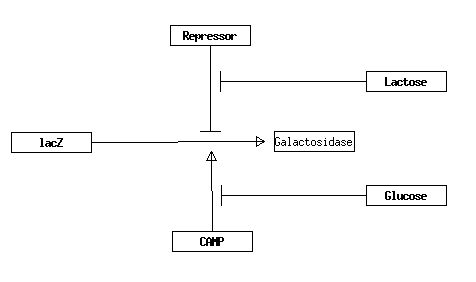
\includegraphics[scale=0.4]{lac_m0001.png}
\end{center}
\caption{Sample toy graph, exogenous variables are in bold font,
  endogenous are in regular font} 
\label{fig:lac3}
\end{figure}

The solution found by the system will be written to the shell:
\begin{verbatim}
Original set:
(lacZ,true)(Repressor,true)(Lactose,true)(Glucose,false)(CAMP,true)
(lacZ,true)(Repressor,false)(Lactose,true)(Glucose,false)(CAMP,true)
(lacZ,true)(Repressor,false)(Lactose,false)(Glucose,false)(CAMP,true)
Reduced set:
(CAMP,true)(Glucose,false)(Lactose,true)(lacZ,true)
(CAMP,true)(Glucose,false)(Repressor,false)(lacZ,true)
\end{verbatim}
Each of the ``original set'' rows corresponds to a complete assignment
of initial values to the exogenous variables that imply the query
(i.e. Galactosidase being true at time 3). Each row in the ``reduced set''
corresponds to a minimal set of assumptions  justifying the query.
\red{When called without the {\tt -orig} option, P3M just shows the
  number of original sets, followed by the reduced sets, like above.}

The values of the exogenous variables are also displayed in the
graphical window: true values are in green, false values in red, and
unset (or don't care) values remain black (see
Figure~\ref{fig:lac4}). 

\begin{figure}[h]
\begin{center}
  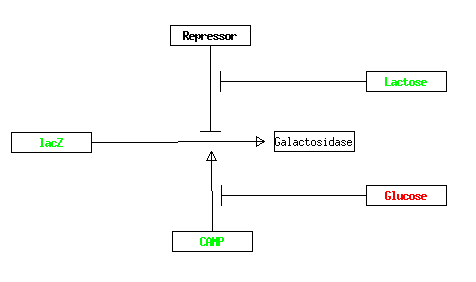
\includegraphics[scale=0.3]{lac_m0002.png}
  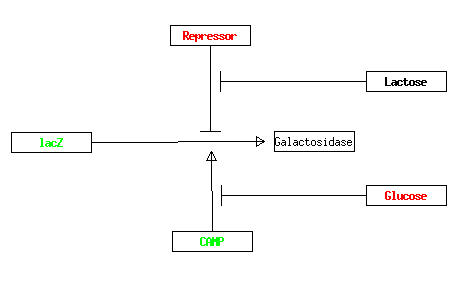
\includegraphics[scale=0.3]{lac_m0003.png}
\end{center}
\caption{The two possible solutions, the colors of the exogenous
  variables depend on their truth values} 
\label{fig:lac4}
\end{figure}


The 'i'  key can be pressed to save an image of the current graph,
the 'n'  key can be used to go to the next set of variables values,
 and the 'p'  key can be used to go back to the previous
set. The 'g'  key exits the current step. 
\hide{%%%%%%%%%%%
Note that in some cases there are more reduced sets.
For instance, p3m -filename lac3 -grounding 3 -query +Galactosidase\(3\) 
gives:
\begin{verbatim}
Original set:
(lacZ,true)(Repressor,true)(Lactose,true)(Glucose,false)(CAMP,true)
(lacZ,true)(Repressor,false)(Lactose,true)(Glucose,false)(CAMP,true)
(lacZ,true)(Repressor,false)(Lactose,false)(Glucose,false)(CAMP,true)
Reduced set:
(CAMP,true)(Glucose,false)(Lactose,true)(lacZ,true)
(CAMP,true)(Glucose,false)(Repressor,false)(lacZ,true)
\end{verbatim}
}%%%%%%%%

If the query is already a consequence of the graph encoding, the
system notifies it. And it also notifies when no solution is
found. These are cases where graph updating may be reasonably asked for. 


\subsection{Graph updating}

When called with the {\tt -graph} option, the system tries at first to
find explanations for the given query without modifying the graph. If
one is found, it notifies the user that there is no need to build a
supergraph.
Otherwise, when no solution can be found, it produces all the possible
ways to obtain a new graph by adding, removing
or modifying a single link. The graph querying task is then invoked on
each of them, and, when a solution can be found, the new graph is
displayed along with the assumptions on initial values that can
explain the query.

\begin{figure}[htb]
\begin{center}
  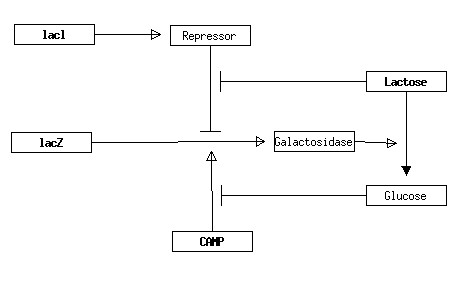
\includegraphics[scale=0.3]{lac0001.png}
  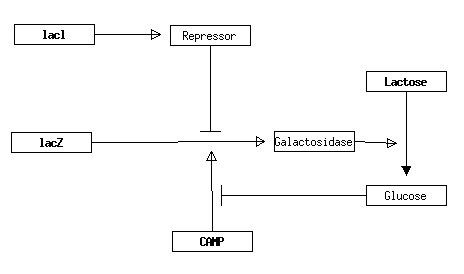
\includegraphics[scale=0.3]{lac_r.png}
\end{center}
\caption{The  lac operon graph (left side), and the same graph without
  the inhibition link (right side)}
\label{fig:supergraph}
\end{figure}

To explain the behaviour of the system for graph updating, we are
going to use the correct form of the graph representing the lac
operon, but with one inhibition missing (see
Figure~\ref{fig:supergraph}). 
In order for P3M to perform graph updating, it can be called as
follows:
%The correct invocation is:
\begin{verbatim}
p3m -filename lac_r -grounding 3 -query +Glucose\(3\) -graph 
    -assumed +lacl+lacZ+CAMP~Repressor~Galactosidase~Glucose
\end{verbatim}
The users can ask the system to save the image by pressing the 'i' key,
before proceeding. When they press the 'g' key, the system goes on
computing other possible graphs that might be solutions. 
Two results among the 144 possible ones are displayed in Figure~\ref{fig:supergraph2}.
\begin{figure}[htb]
\begin{center}
  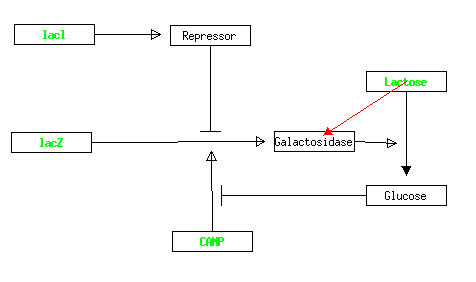
\includegraphics[scale=0.3]{lac_r0004.png}
  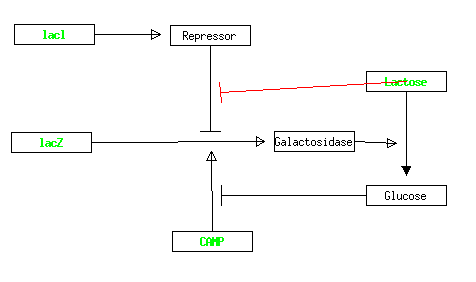
\includegraphics[scale=0.3]{lac_r0005.png}
\end{center}
\caption{Two solutions proposed by the system, the ``correct'' one is on the right.}
\label{fig:supergraph2}
\end{figure}





\end{document}

